\chapter{Evaluation}\label{C:evaluation}

This evaluation will evaluate the the success of the designed and implemented components in achieving their specified requirements as outlined in \Cref{C:design}.


\section{PWM Generation}\label{S:pwm_gen_eval}

It was specified in \Cref{S:pwm_gen_design} that a successful PWM generator subsystem must be capable of duty cycle variation with a resolution of 1.25\%, as specified by requirements 2 \& 3. The successful subsystem must also be capable of varying the switching frequency between 1kHz \& 100kHz with a resolution of 200Hz, as specified by requirements 4, 5, \& 6. 

\subsection*{Duty Cycle Variation}

The design discussed in \Cref{S:PWM_digital_design} outlines it's capabilities for selectable PWM duty cycle, with a resolution of 0.2\%. This precision was verified through visual inspection of oscilloscope measurements at various selected duty cycles, as well as numerically, plotting each targeted duty cycle against the systems output.\\

\subsection*{Switching Frequency Variation}

The design discussed in \Cref{S:PWM_digital_design} outlines it's capabilities for selectable PWM frequency between 1Hz, \& 125kHz. This frequency range was verified through visual inspection of oscilloscope measurements at various selected frequencies across the designed range. 

\begin{figure}[H]
    
    \centering
    \begin{subfigure}{0.45\textwidth}
        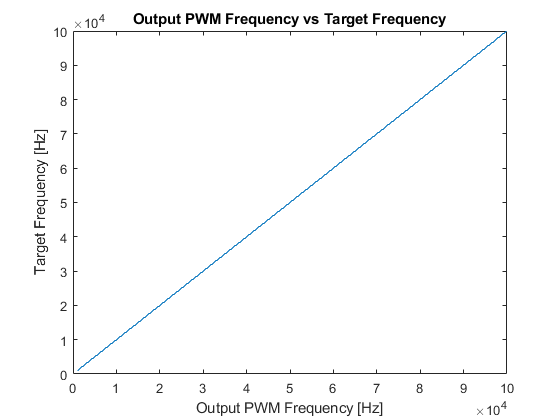
\includegraphics[width=\columnwidth]{pwm/frequency/frequency_range.pdf}
        \subcaption{Output PWM frequency plotted against target frequency}
    \end{subfigure}
    \begin{subfigure}{0.45\textwidth}
        \includegraphics[width=\columnwidth]{pwm/frequency/frequency_error.pdf}
        \subcaption{Output PWM frequency error as a percentage of target frequency}
    \end{subfigure}
    \caption{PWM frequency selection}
    \vspace{-10pt}
    \label{F:pwm_frequency_eval}
\end{figure}

It was also specified that the design would provide a PWM frequency selection error of no more than 200Hz for a provided frequency. This was evaluated numerically by plotting the target output frequency against the systems provided output, and can be seen in \Cref{F:pwm_frequency_eval} (a). To allow for easier visualisation of this error, it was calculated and plotted as a percentage of the target frequency \Cref{F:pwm_frequency_eval} (b). From this data, it was found that the maximum output frequency error of the system was 64Hz, or 0.064\% of the target output.\\

\subsection{PWM Generator Subsystem Evaluation}

The PWM generator subsystem was required to provides a duty cycle selection resolution of at least 1.25\%, and a frequency selection resolution of at least 200Hz, across the 1kHz to 100kHz range. The performed tests show that the implemented subsystem meets these specifications, providing a duty cycle selection resolution of 0.02\%, and a frequency selection resolution of 64Hz.  For the full range of PWM duty cycle and frequency test, measurements, and plots, refer too \Cref{A:digital_PWM}


\section{System State Sensing}\label{S:current_sense_eval}

It was specified in \Cref{S:sensing_design} that a successful state sensing subsystem will provide two sensing elements. The first, an voltage sensor capable of measuring voltages between 3V \& 10V with a resolution of 150mV, specified by requirements 2 \& 3. The second, an inductor current sensor capable of measuring average current and the peak current ripple with a resolution of 15mA, for frequencies between 1kHz \& 100kHz, as specified by requirement 4, 5, 6, \& 7.

\subsection{Output Voltage Sensing}

The design discussed in \Cref{S:v_sense_design} outlines it's capability of measuring a DC voltage between 3V \& 10V, with a measurement resolution of 2.5mV. This measurement precision was evaluated by comparing a selection of known input voltages between 3V and 10V to their measured outputs from the implemented design.\\

From this testing it was identified that a final precision of 10mV was achieved by the design, with signal noise from the ADC presenting as the main design limitation. Although the evaluated resolution of the design does not meet it's designed specification, it still provides a resolution 15 times greater than required.


\subsection{Inductor Current Sensing}

\subsection*{Average Inductor Current}

The design discussed in \Cref{S:avg_current_design} outlines it's capability to provide an average current measurement for frequencies between 1kHz and 100kHz, with a resolution of 244$\mu$A. The frequency range and resolution were evaluated by comparing a selection of known input voltages between 100mV and 3V to their measured outputs from the implemented design. This was then repeated for frequencies of 1kHz, 50kHz, and 100kHz.\\ 

From this testing it was identified that a final precision of 3.5mV was achieved by the design across all frequencies, with similar design limitations as the output voltage sensing. This provided a final average current measurement resolution of 1.1mA.


\subsection*{Peak Inductor Current}

The design discussed in \Cref{S:current_sense_sample_and_hold_design} outlines it's capability to provide a peak current measurement for frequencies between 1kHz and 100kHz, with a resolution of 15mA. As discussed in \Cref{S:peak_current_implementation}, the operation of the original design did not approach the resolution suggested by the simulations, and as such a redesign was undertaken to improve this. 

The precision and functional frequency range of both the initial and final designs were evaluated and compared. In this evaluation, a known peak to peak voltage was input to the design, and compared to it's output DC voltage for a range of frequencies from 1kHz to 100kHz. This was then repeated for input voltages of 150mV, 500mV, and 1500mV, spanning the entire possible input range from the system. An oscilloscope screenshot of this testing for an input of 500mV, and frequencies of 10kHz and 100kHz can be seen in \Cref{F:peak_detect_scope}.

\begin{figure}[H]
    \centering
    \begin{subfigure}{0.45\textwidth}
        \includegraphics[width=\columnwidth]{current_sense/peak_comparison_500mV/10kHz_500mV.PNG}
        \subcaption{Initial (Red) \& final (Blue) peak detetor outputs for a 10$kHz$ 500mV triangle input}
    \end{subfigure}
    \begin{subfigure}{0.45\textwidth}
        \includegraphics[width=\columnwidth]{current_sense/peak_comparison_500mV/100kHz_500mV.PNG}
        \subcaption{Initial (Red) \& final (Blue) peak detetor outputs for a 100$kHz$ 500mV triangle input}
    \end{subfigure}
    \caption{Initial and final peak detector design }
    \vspace{-10pt}
    \label{F:peak_detect_scope}
\end{figure}

From this testing, plots comparing the total error of the two designs as a percentage of the input peak to peak signal were generated, and can be seen in \Cref{F:peak_detect_eval}. From these plots it can be observed that there is an increase in the total error for both designs as the input frequency increases, and a decrease in the total error as the input ripple increases. It can also clearly be seen that the final design provides substantially lower error for all input frequencies and peak to peak values, with a largest recorded error of 8.9\% when operating at the minimum input ripple and maximum frequency.   

\begin{figure}[H]
    \centering
    \begin{subfigure}{0.45\textwidth}
        \includegraphics[width=\columnwidth]{current_sense/error/initial_design_error.pdf}
        \subcaption{Initial design peak current sensing error as a percentage of actual peak current against frequency}
    \end{subfigure}
    \begin{subfigure}{0.45\textwidth}
        \includegraphics[width=\columnwidth]{current_sense/error/final_design_error.pdf}
        \subcaption{Final design peak current sensing error as a percentage of actual peak current against frequency}
    \end{subfigure}
    \caption{Initial and final peak current sensing design, percentage of actual peak current against frequency}
    \vspace{-10pt}
    \label{F:peak_detect_eval}
\end{figure}

From this testing it was identified that a worst case precision of 13.35mV was achieved by the design with an 100kHz input of 150mV peak to peak. After conversion, this provided a worst case peak current measurement resolution of 4.45mA. 

\subsection{State Sensing Subsystem Evaluation}

The state sensing subsystem was required to provide measurements of the buck converters output voltage to a resolution of 150mV, as well as inductor average current and peak current ripple measurements across the 1kHz to 100kHz range to a resolution of 15mA. The performed tests show that the implemented subsystem meets these specifications. This subsystem provides an output voltage measurement resolution of 10mV, an average current sensing resolution of 1.1mA, and a worst case peak ripple sensing resolution of 4.45mA. For the full range of testing, measurements, and plots, refer too \Cref{A:peak_detector}.


\section{Control System}\label{S:control_eval}

It was specified in \Cref{S:control_design} that a successful control subsystem will ensure a steady state error of no more than $\pm$5\% across the output range of 3V to 10V, as specified by requirement 3. It can be noted that the success of this control subsystem relies heavily on the designed specifications of the PWM generator subsystem to implement the selected duty cycle and frequency, as well as the state sensing subsystem to provide reliable and accurate feedback. 

\subsection*{Output Voltage Control}

The design discussed in \Cref{S:output_control_design} outlines it's capability to provide an output steady state error of 23mV, or $\pm$0.78\%. This implemented controller was evaluated using a number of methods, characterising the subsystems steady state error and step response across the across the 3V to 10V output range, as well as the controllers supply change rejection.\\

The step response of the system was evaluated by selecting a system output of 0V DC, and then providing supplying an output target voltage step between 1V DC and 10V DC. From these tests it was observed that there was no output overshoot from the control system, and a consistent settling time of 84ms was observed for all step input values. Oscilloscope screenshots of this controller response can be seen in \Cref{F:control_step}. 

It was also observed from these tests that the designed steady state error of $\pm$0.78\% was achieved, with small output fluctuations of 23mV noticeable in \Cref{F:control_step} (a).

\begin{figure}[H]
    \centering
    \begin{subfigure}{0.45\textwidth}
        \includegraphics[width=\columnwidth]{control/step_response/voltage_control_0-3.PNG}
        \subcaption{Buck converter output voltage controller 3V step response}
    \end{subfigure}
    \begin{subfigure}{0.45\textwidth}
        \includegraphics[width=\columnwidth]{control/step_response/voltage_control_0-10.PNG}
        \subcaption{Buck converter output voltage controller 10V step response}
    \end{subfigure}
    \caption{Buck converter output voltage controller step response for full output voltage range}
    \vspace{-10pt}
    \label{F:control_step}
\end{figure}

The controller response to supply voltage changes was evaluated by allowing the controller to achieve a steady state, and then varying the input supply between values of 6V and 16V respectively. From these tests it was observed that the controller was consistently able to return the output to it's steady state within a period of 250ms. It was also observed that the designed converter was capable of providing any specified output between 1V and 10V across the full tested supply range, so long as the requested output was at least 500mV below the current supply.

\begin{figure}[H]
    \centering
    \begin{subfigure}{0.45\textwidth}
        \includegraphics[width=\columnwidth]{control/variable_input/VCC-step_12-8.PNG}
        \subcaption{Buck converter output voltage controller response to -4V supply transition}
    \end{subfigure}
    \begin{subfigure}{0.45\textwidth}
        \includegraphics[width=\columnwidth]{control/variable_input/VCC-step_8-12.PNG}
        \subcaption{Buck converter output voltage controller response to 4V supply transition}
    \end{subfigure}
    \caption{Buck converter output voltage controller response to varied input supply}
    \vspace{-10pt}
    \label{F:Control_variable_input}
\end{figure}


\subsection{Control Subsystem Evaluation}

The control subsystem was required to ensure that the buck converters output voltage steady state error was no larger than $\pm$5\% across the output range of 3V to 10V. The performed tests show that the implemented sub system meets these specifications. This subsystem has been proven to provide an output voltage steady state error of $\pm$0.78\% across it's full output range, while also providing additional functionality of input supply rejection. This shifts the operating input supply range of all subsystems within this project to between 8V and 16V, as opposed to the static 12V initially specified in requirement 1. 

For the full range of testing, measurements, and plots, refer too \Cref{A:control}.